\documentclass[12pt,a4paper]{article}
\usepackage{anziamjedraft}
\usepackage{bm}

\title{Patch dynamics for macroscale modelling in one dimension}

\author{J.~E. Bunder}
\address{School of Mathematical Sciences, University of Adelaide, South Australia~5005, \textsc{Australia}}
\mailto{judith.bunder@adelaide.edu.au}
\author{A.~J. Roberts}
\address{School of Mathematical Sciences, University of Adelaide, South Australia~5005, \textsc{Australia}}

\begin{document}

\maketitle

\begin{abstract}
We discuss efficient macroscale modelling of microscale systems using patch dynamics. This pilot study effectively homogenises microscale varying diffusion in one dimension. Our `equation free' approach requires that the microscale model need be solved only on small patches of the spatial domain. Suitable Boundary conditions ensure that these patches are well coupled. By centre manifold theory, an emergent closed model exists on the macroscale. Patch dynamics systematically approximates this macroscale model. The modelling is readily adaptable to higher dimensions and to reaction-diffusion equations.
\end{abstract}

\tableofcontents 

\section{Introduction}
\label{sec:intro}
In many applications numerical simulations invoke microscale detail in order to obtain an accurate solution, but only a coarse-grained, or macroscale, solution is required. In principle, a microscale simulation may be obtained over the entire domain, from which macroscale properties can be extracted, but time and memory constraints often make this simulaton impractical or even impossible. For both stochastic and deterministic problems, Givon et al.~\cite{Givon04} reviewed a number of schemes developed to overcome computational limitations inherent in multiscale modelling. 

Here we further develop a multiscale modelling method known as patch dynamics, which makes no attempt to develop a macroscale equation and relies solely on the original microscale computational model.
Due to the lack of a macroscale equation this technique is called equation-free modelling. Hyman~\cite{Hyman05} briefly reviews patch dynamics, while a more detailed review by Kevrekidis and Samaey~\cite{Kevrekidis09} also discusses several physical applications. Samaey et al.~\cite{Samaey10} review the mathematical theory of patch dynamics with numerical examples. For either a deterministic or stochastic problem, the macroscale domain is divided into small, spatially separated patches. The microscale solution is solved within these patches and coupling conditions effectively bridge the gaps in the domain over which no solution is calculated. Each patch contributes one data point to the macroscale solution. In a full implementation, patches are in space-time and projective integration~\cite{Samaey05} simulates forward in time. However, here we limit attention to issues associated with spatial coupling on a one-dimensional domain.

Spatial patch dynamics has been applied to Burgers' equation~\cite{Roberts01}, a generalized advection-diffusion partial differential equation (\textsc{pde})~\cite{Roberts03} and a Ginzburg--Landau \textsc{pde}~\cite{Roberts11}. By utilizing generalized coupling conditions and varying the patch size it was shown, in one-dimension, that the resulting macroscale solution is largely  independent of the patch parameters and systematically approximates the known macroscale dynamics~\cite{Roberts07}. 

Here we consider a one-dimensional diffusion equation with highly variable microscale diffusion with the aim of determining the effectiveness of patch dynamics for a model with significant roughness in the microscale structure. In contrast, the microscale is smooth in all previously mentioned examples and theory. Here, define a microscale lattice with grid points $x_i=ih$, say, with constant spacing $h$. We invoke a diffusive model for the field $u_i(t)$ on the microscale lattice represented by the one-dimensional difference equation
\begin{equation}
\dot{u}_i=\kappa_{i+1/2}(u_{i+1}-u_i)/h^2+\kappa_{i-1/2}(u_{i-1}-u_i)/h^2\label{eq:pde}
\end{equation}
where the diffusivity oscillates through $K$ possible values; that is, the microscale diffusivity is $K$-periodic. Figure \ref{fig:zigzag} illustrates the $K=2$ case. 

Define a macroscale lattices with spacing $H$ and grid points at $x=X_j$. One patch is centered about each macroscale lattice site and indexed by $j$, as shown in Figure \ref{fig:zigzag}. Each patch $j$ is associated with a macroscale solution $U_j(t)$, where $U_j$ is some measure, defined later, of the microscale field $u_i$ in the $j$th patch. It is well established, by homogenization~\cite{Knapek98}, that the effective macroscale equation is
\begin{equation}
\dot{U}_j\approx \kappa(U_{j+1}-2U_j+U_{j-1})
\end{equation}
where $\kappa$ is the harmonic average of the microscale diffusivities. We seek to go beyond this macroscale homogenization in two ways: firstly, to higher accuracy; and secondly, to develop coupling conditions that apply to more general dynamics other than straightforward diffusion. 

\begin{figure}
\begin{center}
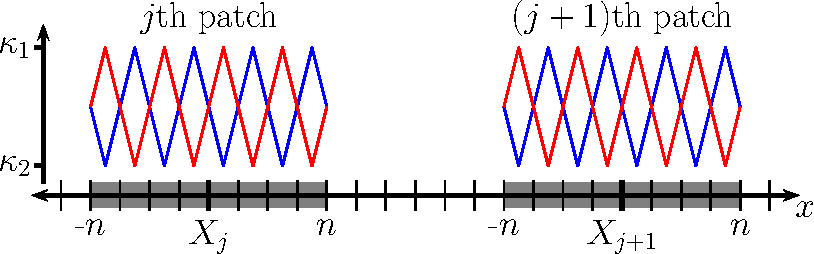
\includegraphics[width=10cm]{zigzagk3}
\caption{The $j$th and $(j+1)$th patches, indicated by the shaded parts of the $x$ axis and centred about the macroscale coordinates $X_j$ and $X_{j+1}$. The macroscale lattice points are marked by thick lines along the $x$ axis, while the microscale lattice points are marked by fine lines.
Here, $K=2$ and $n=4$. The two possible ensembles are indicated by the red and blue lines.}
\label{fig:zigzag}
\end{center}
\end{figure}

Clearly there are many parameters in our patch dynamics scheme, including the width of the patch, the relative scale of the macroscale and microscale lattices and the number of diffusivity periods within each patch. For each microscale configuration there is a set of ideal patch geometries which best approximate the analytic solution. However, we are developing a generic numerical model which is intended to be applicable to numerous unrelated problems and therefore do not want to rely on prior knowledge of the microscale model. With this in mind, we aim to establish the accuracy of patch dynamics for any generic patch, and note some tricks which improve the accuracy without relying on presupposing the microscale model. For example, it is impractical to know the phase of the microscale diffusivities relative to the patches, but without this knowledge the patch dynamics may produce a solution which does not have the same symmetry as the original microscale model. To obtain the correct symmetry in our patch dynamics scheme we simultaneously evaluate several possible ensembles of the diffusivities. For example, when $K=2$ there are two possible ensembles, as shown in Figure \ref{fig:zigzag}. Further details concerning multiple ensembles are discussed later. 


\section{Analytic macroscale modelling}
\label{sec:analytic}

An analytic macroscale solution of Equation (\ref{eq:pde}) determines the accuracy of coupled patch dynamics. In principle an analytic solution exists for any $K$ but in practice only small $K$ cases are straightforward.

\subsection{Two diffusivities}
We consider the case of two diffusivities, $\kappa_{i+1/2}=\kappa_1$ and $\kappa_{i-1/2}=\kappa_2$ for $i$~even. Then, for $i$ even, Equation (\ref{eq:pde}) rewritten in matrix form is 
\begin{equation}
\begin{bmatrix}
\dot{u}_i\\
\dot{u}_{i+1}
\end{bmatrix}=\frac{1}{h^2}\begin{bmatrix}
-\kappa_2-\kappa_1 & \kappa_1+\kappa_2\varepsilon ^{-2}\\
\kappa_1+\kappa_2\varepsilon ^2 & -\kappa_1-\kappa_2
\end{bmatrix}\begin{bmatrix}
u_i\\
u_{i+1}
\end{bmatrix}\label{eq:matrix}
\end{equation}
where  $\varepsilon $ is the step operator on the microscale lattice defined by $\varepsilon u_i=u_{i+1}$. Straightforward `operator' algebra gives the eigenvalues of the above $2\times 2$ matrix as
\begin{equation}
\lambda_{\pm}=-2\kappa_a\left(1\mp \sqrt{1+\kappa\mu^2\delta^2/\kappa_a}\right)
\end{equation}
where $\kappa=2\kappa_1\kappa_2/(\kappa_1+\kappa_2)$ is the harmonic mean and $\kappa_a=(\kappa_1+\kappa_2)/2$ is the algebraic mean of the diffusivities. Here,  the microscale difference operator $\delta=\varepsilon ^{1/2}-\varepsilon ^{-1/2}$ and the microscale mean operator $\mu=(\varepsilon ^{1/2}+\varepsilon ^{-1/2})/2$ are, like the step operator, both defined relative to the microscale lattice.

Macroscale solutions vary slowly on the microscale. For stationary solutions the operator $\mu^2\delta^2$ is small, specifically $\mu^2\delta^2u_i=(u_{i+2}+u_{i-2}-2u_i)/4\ll u_i$. Given that $\kappa\leq \kappa_a$, eigenvalue $\lambda_-\approx -4\kappa_a$ is negative and eigenvalue $\lambda_+\approx \kappa\mu^2\delta^2$ is small. Over macroscale times the dynamics of this system are dominated by that of the eigenvalue of smallest magnitude, $\lambda_+$, that is, $u_i\sim e^{\lambda_+ t/h^2}$. 
The long term dynamics of the slowly varying solutions are thus representable on the macroscale grid as the macroscale evolution
\begin{align}
\dot{U}_j=&\lambda_+U_j/h^2\nonumber\\
=&\frac{\kappa}{h^2}\left[\delta^2+\frac{1}{4}\left(1-\frac{\kappa}{\kappa_a}\right)\delta^4-\frac{\kappa}{8\kappa_a}\left(1-\frac{\kappa}{\kappa_a}\right)\delta^6\right.\nonumber\\
&{}\left.-\frac{\kappa}{64\kappa_a} \left(1-\frac{6\kappa}{\kappa_a}+\frac{5\kappa^2}{\kappa^2_a}\right)\delta^8+O(\delta^{10})
\right]U_j\label{eq:g}
\end{align}
where the expansion of the eigenvalue uses the operator identity $\mu^2=1+\delta^2/4$. 

\subsection{More than two diffusivities}

In general, the analogue of Equation (\ref{eq:matrix}) for $K>2$ is to write Equation (\ref{eq:pde}) in the matrix form $\dot{{\bf u}}=M{\bf u}/h^2$, where ${\bf u}=(u_i,u_{i+1},\ldots,u_{i-1+K})$ and the nonzero elements of the $K\times K$ matrix $M$ are
\begin{alignat}2
M_{i,i}=&-\kappa_{i-1}-\kappa_i,\qquad  &M_{i,i+1}=&M_{i+1,i}\kappa_i,\quad i<K,\nonumber\\
M_{1,K}=&\kappa_K\varepsilon ^{-K},\qquad &M_{K,1}=&\kappa_K\varepsilon ^{K}.
\end{alignat}
The characteristic equation for $K=3$ is
\begin{equation}
\lambda^3+2\lambda^2\sum_{i=1}^3\kappa_i+3\lambda\sum_{i=1}^3\kappa_i\kappa_{i+1}-(\varepsilon ^{3/2}-\varepsilon ^{-3/2})^2\prod_{i=1}^3\kappa_i=0\label{eq:K3}
\end{equation}
and for $K=4$ the characteristic equation is
\begin{multline}
\lambda^4+2\lambda^3\sum_{i=1}^4\kappa_i+\lambda^2\left(3\sum_{i=1}^4\kappa_i\kappa_{i+1}+4\sum_{i=1}^2\kappa_i\kappa_{i+2}\right)\\
{}+4\lambda\sum_{i=1}^4\kappa_i\kappa_{i+1}\kappa_{i+2}-(\varepsilon ^{2}-\varepsilon ^{-2})^2\prod_{i=1}^4\kappa_i=0.
\label{eq:K4}
\end{multline}

The characteristic equations for $K=2,3$ are symmetric in all diffusivities, but for $K=4$ the microscale symmetry is lost by the $\lambda^2$ term in Equation (\ref{eq:K4}), which treats diffusivities differently if they are adjacent to each other.
Such nonsymmetric terms have the interesting consequence that the macroscale evolution subtly depends upon the microscale configuration. Similar nonsymmetric terms arise in the characteristic equations of all $K>3$ cases.

In general the characteristic equation for small $\lambda$ for any $K$ is
\begin{equation}
a({\bm \kappa})\lambda^2+K^2\kappa_g^K/\kappa\lambda-(\varepsilon^{K/2}-\varepsilon^{-K/2})^2\kappa_g^K+O(\lambda^3)=0
\end{equation}
for some function of the diffusivities $a({\bm \kappa})$ and where $\kappa_g=(\prod_i^K\kappa_i)^{1/K}$ is the geometric mean and $\kappa$ is the harmonic mean of all diffusivities. 
Using
\begin{equation}
(\varepsilon^{K/2}-\varepsilon^{-K/2})^2=K^2\delta^2[1+(K^2-1)/12\delta^2]+O(\delta^6),
\end{equation}
the eigenvalue of smallest magnitude is
\begin{equation}
\lambda=\kappa\left[\delta^2+\left(\frac{K^2-1}{12}-\frac{a({\bm \kappa})\kappa^2}{K^2\kappa_g^K}\right)\delta^4\right]+O(\delta^6).\label{eq:glargek}
\end{equation}
For $K>3$, the asymmetry in the diffusivities is apparent at $O(\delta^4)$ due to $a({\bm \kappa})$, but the lowest order homogenization is independent of the microstructure arrangement.

\section{Spatial coupling empowers patch dynamics}
\label{sec:numerical}


\begin{figure}
\begin{center}
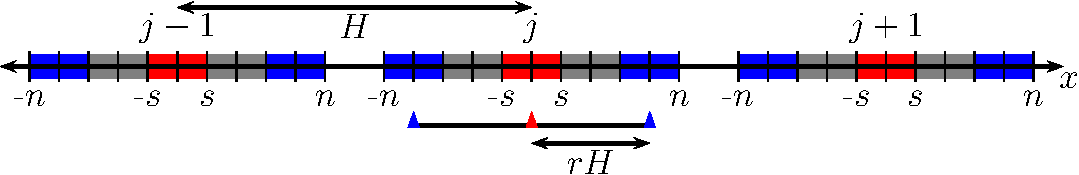
\includegraphics[width=13cm]{1dBC}
\caption{The shaded parts of the $x$ axis represent the $(j-1)$th, $j$th and $(j+1)$th patches, separated by the macroscale distance $H$. Within each patch is a microscale lattice with sites numbered $0,\pm1,\ldots,\pm n$. Each patch has a left and right buffer, shaded blue, both containing $(2s+1)$ lattice sites. The red region is the same width as the buffers and indicates the sites over which the amplitude condition is taken. In this example $n=5$ and $s=1$.}
\label{fig:1dBC}
\end{center}
\end{figure}

As illustrated in Figures \ref{fig:zigzag} and \ref{fig:1dBC}, identical, discrete patches are defined about each macroscale lattice point~$X_j$. Each patch contains $(2n + 1)$ microscale lattice points, for integer~$n$, and therefore has width $2nh$. As the patches must be separated, $nh < H$\,.  We rename the microscale dynamics so that $u_{j,i}(t)$~denotes the microscale field at the point $x=X_j+ih$ of the $j$th~patch for $|i|\leq n$\,.  Our aim here is to develop good coupling between the patches that recovers the correct macroscale dynamics~(\ref{eq:glargek}), and not just the leading order homogenisation.  Such coupling is necessary to empower future simulations to faithfully model microscale dynamics.

One of the assumed characteristics of the macroscale modelling is that we do not know the full details of the microscale structure.  We may know the structure of a sample (via a rock core for example), but we do not know the phase of that structure in the patches.  In this pilot study we therefore seek a macroscale model of the entire ensemble of realisations of phases.  However, here the analytic solution~(13) shows that the macroscale dynamics is slightly different for different microscale configurations.  Thus, we focus on the most straightforward case where the ensemble is over all configurations with the same macroscale model.  By translational and reflectional symmetry this ensemble consists of the $2K$~realisations where the microstructure is shifted in phase, and is reflected.   In this pilot study we model this ensemble over phase shifts and reflections, not just one realisation, and not the full ensemble.


\subsection{Patch coupling and amplitude conditions}
\label{sec:BC}

The patches shown in Figures~\ref{fig:zigzag} and \ref{fig:1dBC} need boundary conditions.  These come by coupling a patch with its near neighbours.  However, practical algorithms implementing patch dynamics couple patches via so-called `buffers' on the edge of each patch: as indicated in Figure~\ref{fig:1dBC}, we find such buffers useful.  The coupling between patches is implemented by the macroscale information specifying the average of the microscale field in the buffers of each patch.
We need to choose the macroscale `grid' values to be the corresponding average over the central region of each patch.  Thus we choose to measure the amplitude of the field in the $j$th~patch by the average over the $(2s+1)$ microscale lattice sites at the centre of the patch:
\begin{equation}
U_j=\left\langle\sum_{i=-s}^su_{j,i,e}/(2s+1)\right\rangle\label{eq:amp2}
\end{equation}
where the subscript $e$ refers to the ensemble and $\langle\ldots\rangle$ denotes the ensemble average. Similarly, the boundary conditions for the buffered patch are
\begin{equation}
\sum_{i=n-2s}^nu_{j,\pm i,e}/(2s+1)=U_j+\sum_{k=1}^{\Gamma}\left(\prod_{l=0}^{k-1}(r^2-l^2)\right)\gamma^k\frac{\pm (2k/r)\bar{\mu}\bar{\delta}^{2k-1}+\bar{\delta}^{2k}}{(2k)!}U_j\label{eq:bc2}
\end{equation}
with coupling strength $\gamma$ and half patch width $rH=(n-s)h/H$. The width is measured from the centre of the patch $i=0$, to the centre of either buffer $i=\pm(n-s)$, as shown in Figure \ref{fig:1dBC}. Note that we have one amplitude condition for all ensembles, and two boundary conditions for each ensemble. 
 
The boundary conditions are dependent on the macroscale operators $\bar{\mu}$ and $\bar{\delta}$, but the analytic solution (\ref{eq:g}) of the evolution is dependent on the microscale operator $\delta$. To derive the relationship between the microscale and macroscale operators, note that one step along the macroscale lattice corresponds to $(n-s)/r$ steps along the microscale lattice since $H=h(n-s)/r$, and therefore $\bar{\varepsilon}^{\pm 1}=\varepsilon ^{\pm(n-s)/r}$. Using this relationship we find
\begin{align}
\bar{\delta}^2=\sum_{l=1}^{\infty}\frac{1}{l!}\left[\prod_{k=0}^{l-1}\left(\frac{n-s}{r}-k\right)\right]\left[(\mu\delta+\delta^2/2)^l+(-\mu\delta+\delta^2/2)^l\right].
\end{align}



\subsection{Slow manifold of macroscale patch dynamics}
\label{sec:results}
We solve Equation (\ref{eq:pde}) with computer algebra to determine the evolution $\dot{U}_j$ and the fields for each ensemble $u_{j,i,e}$ within the $j$th patch.  This is achieved by simultaneously solving Equation (\ref{eq:pde}) for all $|i|<n$ and all ensembles $e$ with two boundary conditions for each ensemble, given by Equation (\ref{eq:bc2}), and one amplitude condition, given by Equation (\ref{eq:amp2}).


We find that the slow manifold macroscale models obtained from patch dynamics are generally dependent on the choice of patch width, controlled by $n$, and buffer width, controlled by $s$, but not the ratio between patch width and macroscale lattice spacing $r$. The lack of dependence on $r$ is expected as a rescaling of the macroscale should not affect the long term evolution.  Here we only discuss $K=2$ in detail and a special case for $K>2$.
\subsubsection{Two diffusivities}

When $n-s$ is even, $2|(n-s)$, the numeric solution is exact when $\gamma=1$, to the same order as the boundary conditions $O(\gamma^{\Gamma})$. For example, when $\Gamma=3$, computer algebra finds the slow manifold, macroscale evolution to be
\begin{equation}
\dot{U}_j=\frac{\kappa}{h^2}\left[\gamma\delta^2+\frac{1}{4}\left(1-\frac{\kappa}{\kappa_a}\right)\gamma^2\delta^4-\frac{\kappa}{8\kappa_a}\left(1-\frac{\kappa}{\kappa_a}\right)\gamma^3\delta^6+O(\gamma^4)
\right]U_j
\end{equation}
which, when $\gamma=1$ is identical to the analytic solution in Equation (\ref{eq:g}) to errors $O(\gamma^4)$. We have determined that this exact equality between patch dynamics and the complete solution holds at least up to $O(\gamma^?)$. The impart is that numerical simulations implementing the coupling (\ref{eq:bc2}) are faithful to the microscale dynamics to at least $O(\gamma^?)$.

When $2|(n-s)$ is not satisfied patch dynamics does not exactly match the true evolution. Here we only consider up to $O(\gamma^2)$ as higher orders are complicated. For this case the evolution is
\begin{multline}
\dot{U}_j=\frac{\kappa}{h^2}\left[\frac{1}{1-\alpha_1(1-\kappa/\kappa_a)}\gamma\delta^2\right.\\
\left.{}+\frac{1+\alpha_2+\alpha_3(1-\kappa/\kappa_a)}{[1-\alpha_1(1-\kappa/\kappa_a)]^3}\frac{1}{4}\left(1-\frac{\kappa}{\kappa_a}\right)\gamma^2\delta^4 +O(\gamma^3)\right]U_j
\end{multline}
where
\begin{align}
\alpha_1=(n-s)^{-2}(2s+1)^{-2},&\qquad\alpha_2=\alpha_1[4(n-s)^2+2(2s+1)^2-9]/3,\nonumber\\
\alpha_3=&\alpha_1[3-2(2s+1)^{-2}-\alpha_1]/3.
\end{align}
The discrepancy with Equation (\ref{eq:g}) is minimized when $\alpha_{1,2,3}$ are minimized. It is straightforward to show that $\alpha_1$ is minimized when $s=(2n-1)/4$. Figure \ref{fig:alpha} shows that for fixed $n$, $\alpha_{1,2,3}$ are all minimized when $s\approx n/2$ and their minimal values decrease as $n$ increases. 

\begin{figure}
\begin{center}
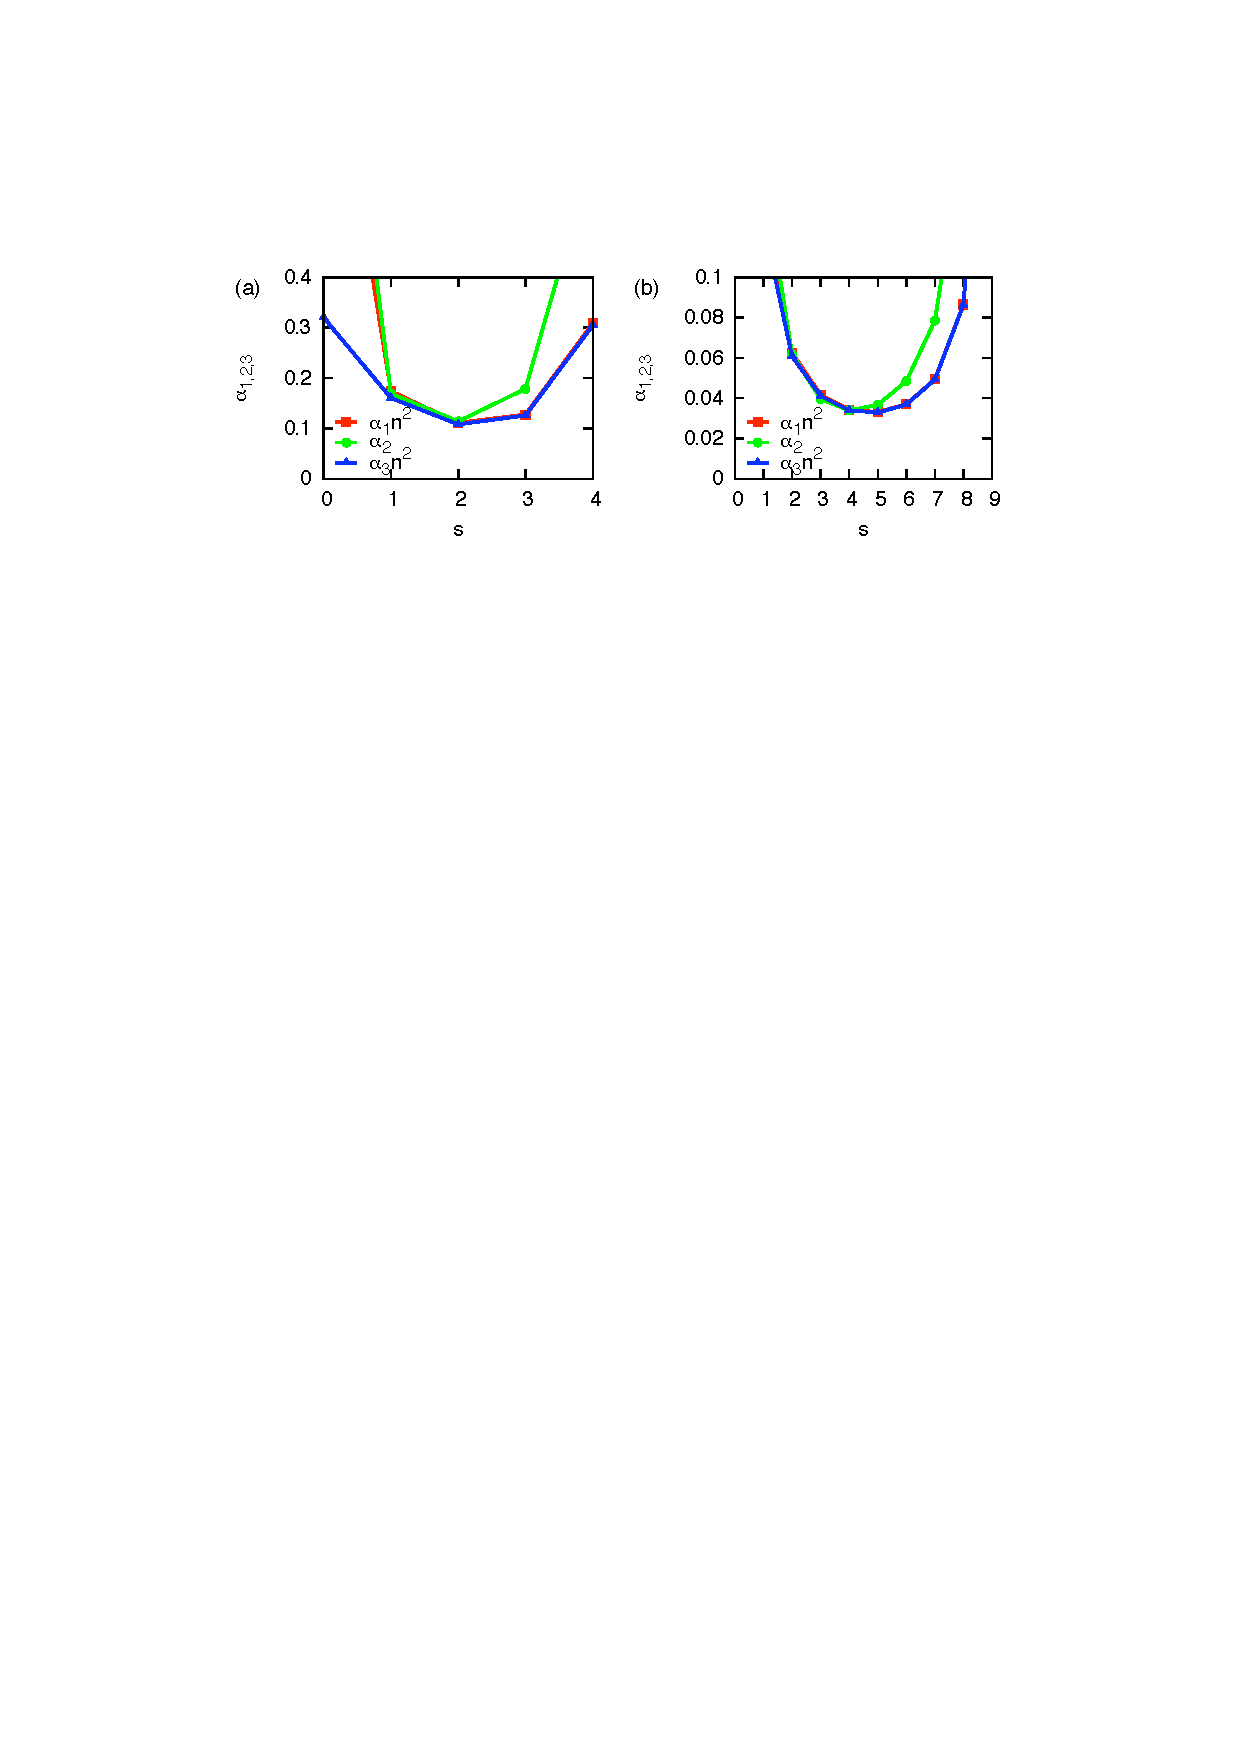
\includegraphics[width=13cm]{alpha}
\caption{Plots of $\alpha_{1,2,3}$ for (a) $n=5$ and (b) $n=10$. Note that $\alpha_{1,3}$ are both scaled by $n^2$. All three curves are minimized for large buffers, when $s\approx n/2$.}
\label{fig:alpha}
\end{center}
\end{figure}

\subsubsection{More than two diffusivities}

In analogy to the $K=2$ case, when $2|(n-s)$, for $K\leq ?$ and $\Gamma=2$ with $K|(n-s)$ computer algebra constructs a slow manifold, macroscale, patch evolution which agrees exactly with Equation (\ref{eq:glargek}) at full coupling $\gamma=1$. Further research is required to determine the accuracy of the slow manifold obtained from patch dynamics when $K|(n-s)$ is not satisfied.

\section{Conclusion}
\label{sec:concl}
For the macroscale modelling of a microscale system with significant microscale roughness, we showed that patch dynamics can provide solutions of arbitrary accuracy. We used the example of a one-dimensional diffusion equation with $K$-periodic microscale diffusivity and compared analytic solutions to the slow manifold modelling of the patch dynamics. To ensure the symmetry of the original model is maintained we simultaneously solved multiple diffusivity ensembles. The accuracy of the patch dynamics modelling depends on the patch geometry as a function of the periodicity $K$ with some geometries reproducing the analytic solution exactly to high order of $\gamma$. However, as we are developing a generic patch dynamics scheme which is intended to be applicable to a wide range of unrelated systems, we cannot assume complete prior knowledge of microscale detail. Therefore, we need to know the errors associated with non-optimal geometries and how best to minimize these errors without resorting to an analysis of the microscale equations. For $K=2$ we found that errors are typically reduced when the patch width is increased and the buffers, over which the boundary and amplitude conditions are averaged, are approximately half the width of the  patch but further research is required to determine optimal parameters for larger $K$. 
\bibliography{../../bibliography/bibliography}
\bibliographystyle{abbrv} 

\end{document} 

Returning to $K=3$, when $3|(s-1)$ but not $3|(n-s)$ with $\Gamma=2$,
\begin{equation}
\dot{U}_j=\kappa\left[\gamma\delta^2+\frac{2(n-s)^3+2(n-s)\pm 1}{3(n-s)^3}\left(1-\frac{\kappa^2\kappa_a}{\kappa_g^3}\right)\gamma^2\delta^4+O(\gamma^3)\right]U_j
\end{equation}
with the alternative signs determined by $3|(n-s\mp 1)$. When $\gamma=1$ this is a good approximation to the analytic solution in Equation (\ref{eq:glargek}) provided $(n-s)$ is large. 
For higher $K$ there do not appear to be any cases analogous to this one. In this special case 
a symmetry again arises in the patch. Here, the pattern of diffusivities on the left of the patch is obtained from the right side of the patch by reflecting about the centre of the ptach and exchanging $\kappa_i\leftrightarrow \kappa_{i+1}$ and leaving $\kappa_{i+2}$ unchanged, for any one $i=1,2,3$ (depending on the chosen ensemble). Such a symmetry does not arise for value of $K$ other than $3$.

When neither $3|(s-1)$ nor $3|(n-s)$ is satisfied and $\Gamma=1$ patch dynamics produces 
\begin{equation}
g=\kappa\left[\mbox{(SOME FUNCTION)}\gamma\delta^2+O(\gamma^2)\right]U_j
\end{equation}



, for example, for $K=5$,
\begin{multline}
\lambda^5+2\lambda^4\sum_{i=1}^5\kappa_i+\lambda^3\left(3\sum_{i=1}^5\kappa_i\kappa_{i+1}+4\sum_{i=1}^5\kappa_i\kappa_{i+2}\right)\\
{}+\lambda^2\left(4\sum_{i=1}^5\kappa_i\kappa_{i+1}\kappa_{i+2}+6\sum_{i=1}^5\kappa_i\kappa_{i+2}\kappa_{i+3}\right)\\
{}+5\lambda\sum_{i=1}^5\kappa_i\kappa_{i+1}\kappa_{i+2}\kappa_{i+3}-(\varepsilon ^{5/2}-\varepsilon ^{-5/2})^2\prod_{i=1}^5\kappa_i=0,
\end{multline} 
and $K=6$,
\begin{multline}
\lambda^6+2\lambda^5\sum_{i=1}^6\kappa_i+\lambda^4\left(3\sum_{i=1}^6\kappa_i\kappa_{i+1}+4\sum_{i=1}^6\sum_{j=2}^3\kappa_i\kappa_{i+j}\right)\\
{}+\lambda^3\left(4\sum_{i=1}^6\kappa_i\kappa_{i+1}\kappa_{i+2}+6\sum_{i=1}^6\sum_{j=2}^3\kappa_i\kappa_{i+j}\kappa_{i+j+1}+8\sum_{i=1}^2\kappa_i\kappa_{i+2}\kappa_{i+4}\right)\\
{}+\lambda^2\left(5\sum_{j=1}^6\kappa_i\kappa_{i+1}\kappa_{i+2}\kappa_{i+3}+8\sum_{i=1}^6\kappa_i\kappa_{i+2}\kappa_{i+3}\kappa_{i+4}+9\sum_{i=1}^6\kappa_i\kappa_{i+2}\kappa_{i+3}\kappa_{i+5}\right)\\
{}+6\lambda\sum_{i=1}^6\kappa_i\kappa_{i+1}\kappa_{i+2}\kappa_{i+3}\kappa_{i+4}-(\varepsilon ^{3}-\varepsilon ^{-3})^2\prod_{i=1}^6\kappa_i=0.
\end{multline} 



The macroscale lattice spacing is $H$ and the microscale lattice spacing is $h$. As illustrated in Figures \ref{fig:zigzag} and \ref{fig:1dBC}, identical, discrete patches are constructed about each macroscale lattice point $X_j$, and the patch about $X_j$ is referred to as the $j$th patch. 
Each patch contains $(2n+1)$ microscale lattice points, for integer $n$ and therefore has width $2nh$. As the patches must be discrete, $nh<H$. 

Using patch dynamics, we only evaluate the microscale Equation (\ref{eq:pde}) within each patch. By coupling these patches together, we obtain a solution for the macroscale evolution. The coupling of the patches is achieved though suitable boundary conditions. In addition, to limit the growth of the microscale fields within a patch, we introduce an amplitude condition. The boundary and amplitude conditions are discussed in Section \ref{sec:BC}. Dividing the domain into patches may destroy the symmetry of the original model. In Section \ref{sec:ensembles} we discuss how this issue may be overcome by considering multiple ensembles. Finally, in Section \ref{sec:results} we present and discuss our numerical solutions. 

\subsection{Multiple ensembles}
\label{sec:ensembles}

Dividing the domain into discrete patches may cause some symmetry in the original microscale model to be lost. For example, when $K=2$ the diffusivity alternates between $\kappa_1$ and $\kappa_2$ and the model, and thus the analytic solution, is symmetric under the exchange of these two diffusivities. However, if the patches do not have the same symmetry as the original microscale model then the numerical solution need not have the correct symmetry. 

To ensure our patch dynamics solution will have the required symmetry, or indeed asymmetry, in the diffusivities we evaluate a number of ensembles simultaneously. While each ensemble has a different solution for $u_{j,i}$, the solution of the microscale field within the $j$th patch, the macroscale evolution $g=\dot{U}_j$ will be identical across all ensembles. For a given value of $K$ there are a total of $K!$ possible ensembles since there are $K!$ possible permutations of the diffusivities. However, in general, as we shall show, we should not include all these ensembles in our numerical model. To determine which of the $K!$ ensembles should be included in our numerical model we analyze the analytic model. 

As noted in Section \ref{sec:analytic}, the characteristic equation (\ref{eq:K4}) for $K=4$ and all higher value of $K$ is not symmetric in all diffusivities and the order in which the diffusivities occur is important. The same is true for higher values of $K$. Therefore, we choose only those ensembles which retain the original ordering of the $K$ diffusivities, although their position may change on the patch. For example, one ensemble begins with $\kappa_1$ on the left of the patch and then $\kappa_2,\kappa_3,\ldots$ across the patch. A second ensemble begins with $\kappa_2$ on the left of the patch, followed by $\kappa_3,\kappa_4,\ldots$, with the diffusivities similarly shifted to created all ensembles of this form. In total there are $K$ such ensembles. 

In the analytic solutions for all $K$ is that there is no favoured direction. All coefficients of powers of $\lambda$ contain only diffusive terms with no direction implied and the  constant term, $(\varepsilon^{K/2}-\varepsilon^{K/2})^2U_j$, treats fields to the left and right of $X_j$ identically. To avoid any favoured direction in the numerical solution we include ensembles which reverse the original direction of the diffusivities, while maintaining the same order. For example, one ensemble begins with $\kappa_K$ on the left of the patch, followed by $\kappa_{K-1},\kappa_{K-2},\ldots$, while a second ensembles begins with $\kappa_{K-1}$ followed by $\kappa_{K-2}\kappa_{K-3},\ldots$, with other ensembles constructed similarly. In total there are $K$ reversed order ensembles. 

In general we must consider $2K$ ensembles in order to maintain the symmetry of the original microscale model. However, for the special case of $K=2$ only two unique ensembles exist. The two ensembles of $K=2$ are shown in Figure \ref{fig:zigzag}. For $K=3$, $2K=K!$, so we must consider all possible ensembles for this case. For $K>3$, however, not all ensembles are required for the numerical solution.


The boundary conditions for the two points at the edge of the $j$th patch, $i=\pm n$, are~\cite{Roberts11}
\begin{equation}
u_{j,\pm n}=U_j+\sum_{k=1}^{\Gamma}\left(\prod_{l=0}^{k-1}(r^2-l^2)\right)\gamma^k\frac{\pm (2k/r)\bar{\mu}\bar{\delta}^{2k-1}+\bar{\delta}^{2k}}{(2k)!}U_j+O(\gamma^{\Gamma+1})\label{eq:bc}
\end{equation}
up to order $\Gamma$ with patch coupling strength $\gamma$ and $rH$ is half the patch width ($r$ being the ratio between half the patch width and the macroscale lattice spacing).
Here, $\bar{\delta}=\bar{\varepsilon}^{1/2}-\bar{\varepsilon}^{-1/2}$ and $\bar{\mu}=(\bar{\varepsilon}^{1/2}+\bar{\varepsilon}^{-1/2})/2$ are the difference and mean operators defined relative to the macroscale lattice with macroscale step operator $\bar{\varepsilon}$ such that $\bar{\varepsilon}U_j=U_{j+1}$. When the patches are uncoupled $\gamma=0$ and the numerical solution is guaranteed, by centre manifold theory, to both exist and be relevant~\cite{Roberts03}. The physical case is restored when $\gamma=1$ and is intended to lie within the region where centre manifold theory remains valid. 

The amplitude condition relates the microscale fields $u_{j,i}$ in the $j$th patch to macroscale fields $U_j$  and effectively limits the growth of the microscale fields. There are many possible amplitude conditions. Perhaps the simplest choice is~\cite{Roberts11}
\begin{equation}
U_j=u_{j,0}.\label{eq:amp}
\end{equation} 

Rather than defining the boundary conditions in terms of the two sites on the edge of the patch, we wish to modify Equation (\ref{eq:bc}) so the boundary conditions are dependent on some average of a number of sites closest to the edges of the patch. These regions over which the boundary conditions are averaged, or buffers, are intended to smooth out any rapid microscale variations thus providing a more accurate approximation of the macroscale evolution. 
For the same reason, we wish to modify the amplitude condition in Equation (\ref{eq:amp}) so that it contains some average over the centre of the patch. In addition, we need to take into account the $2K$ ensembles which need to be simultaneously evaluated. 

We firstly choose a simple amplitude condition based on the average of the $(2s+1)$ microscale lattice sites closest to the centre of the patch,
